\documentclass[11pt]{article}
\usepackage[utf8]{inputenc}
\usepackage{geometry}
\geometry{a4paper, margin=1in}
\usepackage{amsmath, amssymb, amsthm}
\usepackage{graphicx}
\usepackage[hidelinks]{hyperref}
\usepackage[nameinlink]{cleveref}
\usepackage{parskip}

\graphicspath{ {./figs/} }

\title{S2 Coursework: Coal Mining Accident Analysis}
\author{Fred Lawrence - fl482}

\begin{document}

\maketitle

\section*{1. Accident Data}
% Question: Mean rate and cumulative plot
The total number of accidents recorded is $N=191$ over a period of $L=40550$ days. The mean rate of accidents is $0.00471$ accidents/day
or $1.72$ accidents/year.
\[ \bar{\lambda} = \frac{N}{L} \approx 0.0047 \text{ accidents/day.} \]

\begin{figure}[htbp]
    \centering
    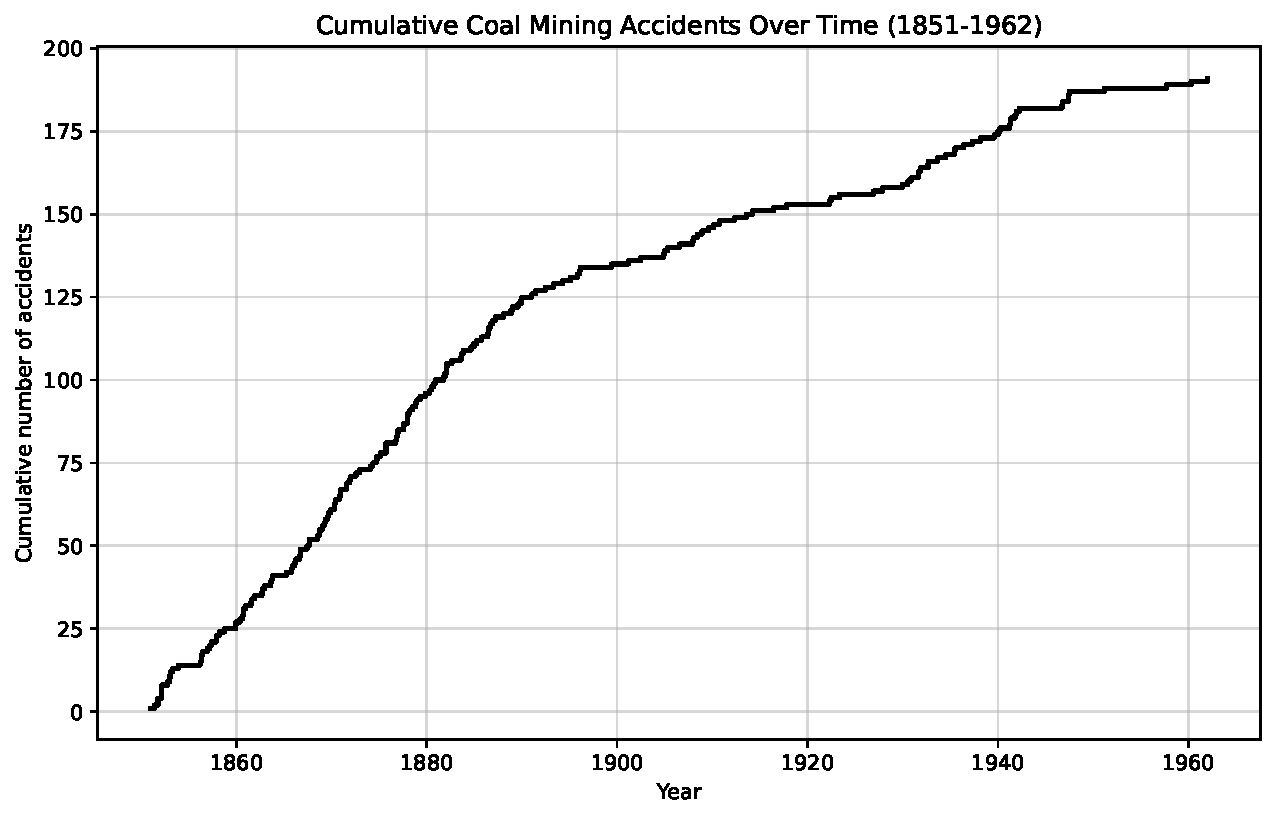
\includegraphics[width=0.8\textwidth]{Ex1a.pdf}
    \caption{Cumulative number of coal mining accidents from 1851 to 1962.}
    \label{fig:1a}
\end{figure}

\section*{2. Priors}
\subsection*{(a) Qualitative Comparison}
% Limit: Under 200 words.
The plain order statistics prior involves drawing $k$ change points from a uniform distribution over the interval $[0, L]$ and then sorting them. This means that the points are independent before sorting and can be clustered tightly together. As shown in \Cref{fig:2a}, the marginal distributions are broad and can peak directly at the boundaries.

The even-numbered prior is constructed by drawing $2k + 1$ points uniformly, sorting them, and then taking the evenly indexed points. This results in a repulsive effect between points, encouraging more evenly spaced change points. It also has the effect of preventing peaks at the boundaries as the first and last points are always odd and therefore always excluded. In \Cref{fig:2a} we can also see that the marginal distributions are more distinctly separated and narrower than those of the plain order priors.
% Word count check: 115 words.

\begin{figure}[htbp]
    \centering
    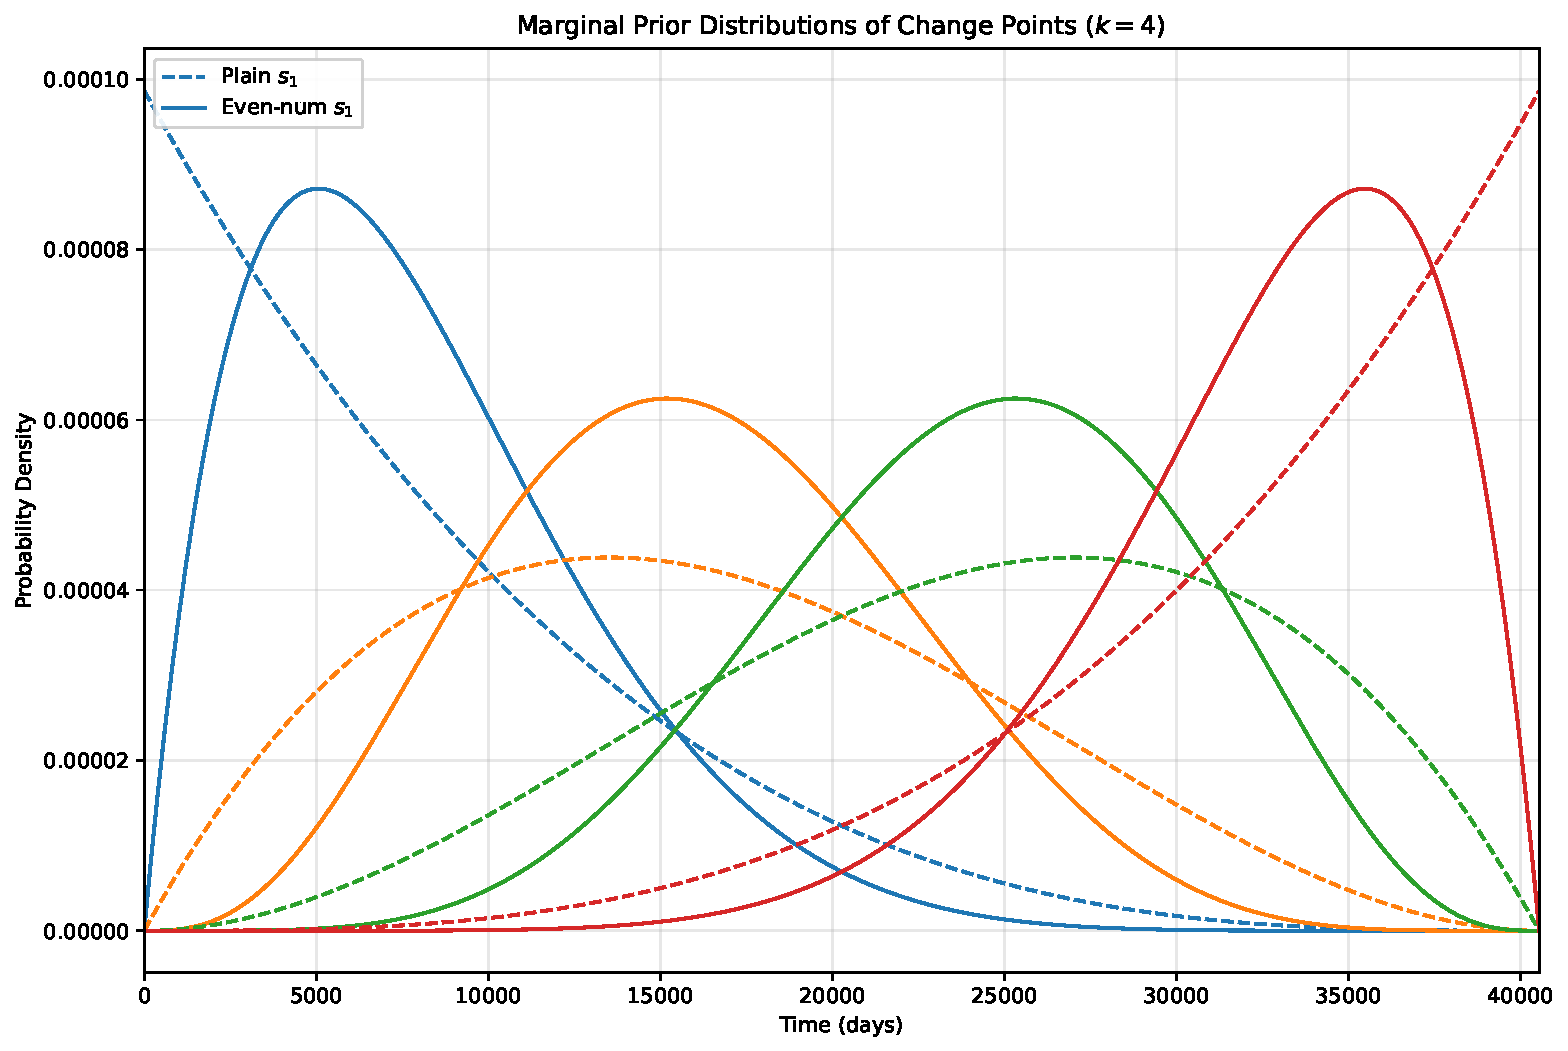
\includegraphics[width=0.8\textwidth]{Ex2a.pdf}
    \caption{Comparison of plain and even-numbered order statistics priors for $k=4$ accross different values of $j$. Plain order priors are shown with a dashed line and even numbered priors with a solid line.}
    \label{fig:2a}
\end{figure}


\subsection*{(b) PDF Derivation}
% Requirement: Show the PDF of the even-numbered order statistics.
To derive the even-numbered pdf we start with the fact that the plain ordered pdf for $2k+1$ points on the unit interval $[0, 1]$ is a constant

$$P(u_{(1)}, u_{(2)}, \dots, u_{(2k+1)}) = (2k + 1)!$$

This is valid only on the strictly ordered region $0 < u_{(1)} < u_{(2)} < \dots < u_{(2k+1)} < 1$.

For the even numbered pdf we only keep even-numbered order statistics $\hat{s}_j = u_{(2j)}$ so must marginalise the plain order pdf over all the other discarded points. We know that the points are ordered and on the unit interval $[0, 1]$ so the integral is

$$P(\hat{s}_1, \dots, \hat{s}_k) = \int_{0}^{\hat{s}_1} \int_{\hat{s}_1}^{\hat{s}_2} \dots \int_{\hat{s}_k}^{1} (2k + 1)! \, du_{(2k+1)} \dots du_{(3)} du_{(1)}$$

Because the integrand $(2k+1)!$ is a constant, each integral becomes the length of the interval between the 2 points on the bounds, or the gap $\hat{g}_j$ between them.

$$P(\hat{s}_1, \dots, \hat{s}_k) = (2k + 1)! (\hat{s}_1)(\hat{s}_2 - \hat{s}_1)\dots(1 - \hat{s}_k)$$

$$=  (2k + 1)! \prod_{j=1}^{k+1} \hat{g}_j$$

We now need to map this from the unit interval $[0, 1]$ to the actual timeline $[0, L]$. We are given the scaling relationship $s_j = L\hat{s}_j$ so can scale the gaps according to $\hat{g}_j = g_j / L$ and substitute this into the equation

$$P(\hat{s}_1, \dots, \hat{s}_k) = (2k + 1)! \prod_{j=1}^{k+1} \left( \frac{g_j}{L} \right)$$

Since $L$ is a constant it can be pulled out of the product

$$P(\hat{s}_1, \dots, \hat{s}_k) = \frac{(2k + 1)!}{L^{k+1}} \prod_{j=1}^{k+1} \left( g_j \right)$$

We must then apply the change of variables formula 

$$P(s_1, \dots, s_k) = P(\hat{s}_1, \dots, \hat{s}_k) \times \left| J \right|$$

where $|J|$ is the Jacobian determinant of the transformation. 

Since $s_j = L \hat{s}_j$, the inverse transformation is $\hat{s}_j = \frac{s_j}{L}$. Taking the derivative of each variable gives $\frac{\partial \hat{s}_j}{\partial s_j} = \frac{1}{L}$. The Jacobian determinant is then given by the product of the derivatives and since there are $k$ points,

$$\left| J \right| = \left( \frac{1}{L} \right)^k = \frac{1}{L^k}$$

This allows us to obtain the final pdf

$$\pi(s_1, s_2, \dots, s_k | M_k) = \frac{(2k+1)!}{L^{2k+1}} \prod_{j=1}^{k+1} g_j$$

$$\pi(s_1, s_2, \dots, s_k | M_k) \propto \prod_{j=1}^{k+1} g_j$$

\section*{3. The constant rate model, $M_0$}
% Requirement: Prior vs Posterior plot and evidence calculation.

\section*{4. The 1 change point model, $M_1$}
\subsection*{(a) MCMC Analysis}
% Limit: Under 300 words.

\subsection*{(b) Savage Dickey Density Ratio}
% Limit: Under 200 words.

\section*{5. The k change point models, $M_k$}
% Requirement: MAP number of change points and inferred rate with uncertainties.

\section*{Declaration of AI Use}
% Requirement: Include a declaration of use of autogeneration tools.
I have used autogeneration tools to assist with code debugging, LaTeX formatting and helping to generate figures. This declaration is made in accordance with the Course Handbook.

\end{document}